\documentclass{article}
\usepackage[utf8]{inputenc}
\usepackage{geometry}
\geometry{letterpaper, portrait, margin=1in}

\title{Traviz: Visualization of Traces in Distributed Systems}
\author{Vaastav Anand \\ vaastav.anand05@gmail.com  \and Matheus Stolet \\ stolet@cs.ubc.ca}

\date{}

\usepackage{natbib}
\usepackage{graphicx}

\begin{document}

\maketitle

\section{Introduction}

Distributed systems form the backbone of many modern applications. The Google search engine,
YouTube, Facebook, and even the mediocre web app built by your neighbor's prodigy kid touches
a distributed system in some way. These systems form much of the mission critical infrastructure
of modern computing and are comprised of multiple nodes with complex communication patterns. Because
of the importance and complexity of distributed systems, it is crucial for the developers building
them to identify performance bottlenecks and visualize different communication patterns. 

Tracing is a technique that allows developers to better understand distributed systems. A trace represents the
path of one request through the system and contains information such as the timing of requests, 
the events executed, and the nodes where these events were executed. Moreover, traces can be used
to identify slow requests and understand the difference between request executions. In this project, we
propose to create a visualization tool that uses data from traces to succintly represent the structure 
and performance of a distributed system. Our tool will allow users to compare the path taken by a group
of requests to the path taken by other requests. We believe that a visualization tool that can represent the
structure of a trace, while also visually encoding releveant performance information, will make distributed
systems more understandable and debuggable.

Both of us have experience with the problem domain. Vaastav has been working on distributed systems for years
and participated in many different projects in the area. Furthermore, his recent research has investigated
tracing in distributed systems. Matheus also has experience with distributed systems through coursework,
research assistanships and graduate research. Tracing is a new topic for him, but he has found it to be
an interesting area that can be useful for debugging and comprehending the interactions of large networks
of computers.

\section{Data}

We have a collection of traces and source code for a couple of different systems. Our traces come from two datasets.
The first dataset is called HDFS and contains the traces from a Haddop file system used for distributed storage 
and big data processing. This dataset has a total of 71,001 traces. The second dataset is called socialNetwork and
was obtained from the DeathStarBench open-source benchmark for cloud microservices. This dataset's traces model
the microservices of a social network composed of multiple individual applications. The socialNetwork dataset has
a total of 22,286 traces. The attributes of both datasets model five different entities: traces, events, hosts,
processes and threads. These entities are illustrated in \ref{fig:entities}.

\begin{figure}
    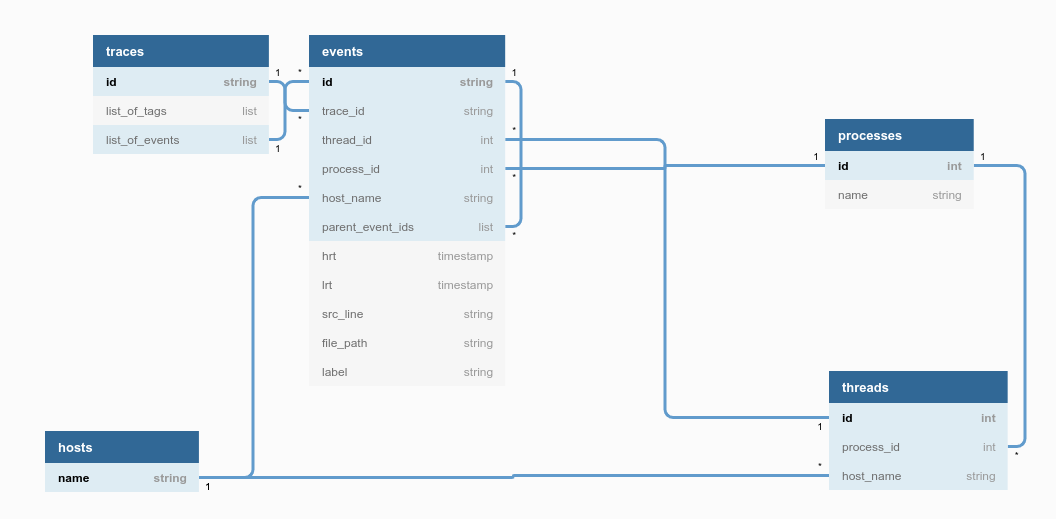
\includegraphics[width=\linewidth]{../data_abstractions.png}
    \caption{The different entities in TraViz.}
    \label{fig:entities}
  \end{figure}

\subsection{Trace}

A trace is a collection of events. It represents a request from a client to a service and shows the path of the
request through the microservice. A trace has three attributes: \textit{id}, \textit{list\_of\_tags}, and \textit{list\_of\_events}.
The \textit{id} of the trace is a categorical attribute used to identify a trace. The \textit{list\_of\_tags} is a list of human defined keywords that serve as
the metadata for the trace. There are on average two tags per trace in both datasets, but the socialNetwork
dataset has a total of 8 different tags and the HDFS dataset has a total of 22285 different tags. The
\textit{list\_of\_events} attribute is a list of the events that happened in a trace. The events in the list
are ordered, with events that caused another event preceding the caused event in the list. The causal relationship
between the events forms a DAG. There are around 100 events per trace in the socialNetwork dataset and 1400 events per trace
in the HDFS dataset.

\subsection{Event}

Events are important things that happen in a system, such as acquiring a lock, sending a request to another server,
or performing an update. In short, events are anything a developer things is useful enough to log. Events have 11
different attributes. They are \textit{id}, \textit{trace\_id}, \textit{thread\_id}, \textit{process\_id}, \textit{host\_name},
\textit{parent\_event\_ids}, \textit{hrt}, \textit{lrt}, \textit{src\_line}, \textit{file\_path}, and \textit{label}. The
\textit{id} is a categorical variable used to uniquely identify an event. The \textit{trace\_id} is another categorical
attribute that indentifies the trace that holds an event. The \textit{thread\_id} is a categorical variable that identifies the
thread that executed the event. The \textit{process\_id} gives the id of the process holding the thread that executed the event.
The \textit{host\_name} gives the name of the machine running the process that executed the event. An event can have at most one
host. The \textit{parent\_event\_ids} attribute is a collection of event ids. Each id maps to a parent event. The ids are used to
create a causal ordering between events. The socialNetwork and HDFS datasets have on average one parent event id per event, but 
can have up to two parent events for one event. 

The \textit{hrt} is a quantitative attribute that stands for high resolution time
stamp, and provides nanosecond level precision for the time an event was initiated. The \textit{lrt} is also a quantitative attribute.
It provides a milisecond level precision low resolution time stamp for the time an event occured. The \textit{src\_line} gives the line
in the source code where an event was logged. The \textit{file\_path} is a categorical attribute that gives the path to the file where 
a programmer logged this specific event. This attribute can be used with the \textit{src\_line} to find the exact line of code of a logged event.
The last attribute in an event is the \textit{label}. The label is a free-form text annotaion that gives a high-level description of the
event. Labels are a meaningful human added annotation for debugging, and there are 2,472 labels in the socialNetwork dataset and 210,957 labels
in the HDFS dataset.

\subsection{Host}

A host represents a node in the distributed system. Hosts encapsulate the processes and threads
that execute the events in a trace. There are 13 different hosts across the social network dataset
and 9 different hosts across the HDFS dataset. The host is identified by a categorical \textit{name} attribute , which is
referenced by events and threads.

\subsection{Process}

The process entity represents a operating system process running on
a host. Processes have a categorical \textit{id} attribute, which is referenced by the events and threads executed in
the process. The process also has a categorical \textit{name} attribute, which gives a human understandable name for the
application running the process. There are around 20 different processes per trace in the socialNetwork
dataset and 18 different processes per trace in the HDFS dataset. There are 13 different process names
in the socialNetwork dataset and 4 different process names in the HDFS dataset.

\subsection{Thread}

The thread entity represents
a kernel or user thread. Distinguishing between both is not important for the purposes of this project, so we
simply see it as the basic unit of execution. Threads have a categorical \textit{id} attribute that identifies a thread
within a trace. Events use the \textit{id} to signal the thread that executed them. It is important to note
that the thread \textit{id} does not match across traces, and the total number of threads is not useful because it's
not possible to correlate them between traces. Each thread also has two more categorical attributes: the \textit{host\_name}
and \textit{process\_id}. These attributes are used to identify the host and process that executed a thread. 

\section{Task}

For this project we want to focus on comparison tasks. Namely, we want to compare the path and performance of different
requests. Each one of our traces represents a request and each event in a trace represents a directed acyclic graph. Our
comparison tasks are meant to compare the structure of the DAGs created by the events in a trace and the duration of a request. 
We want to support three different comparison tasks: one trace against one trace, one trace against many traces, and many traces
against many traces. These tasks will take the form of comparing DAGs against each other.  

\section{Proposed Solution}



\section{Implementation Approach}

Our visualization tool will be a webapp that can be accessed through a browser. We will host a backend written in Go that 
will serve requests from a client. The frontend will be written in javascript. We will use D3 to manipulate the data served
by our backend and create the visualizations necessary to fulfill our comparison tasks.

\section{Schedule}

\section{Related Work}

\end{document}

